\documentclass{article}
\usepackage{amsthm}
\usepackage{graphicx}
\usepackage{ctex}
\usepackage{amsmath}
\usepackage{amssymb} % 添加 amssymb 以支持更多符号
\usepackage{amsfonts}
\usepackage{tikz}
\usepackage{cancel}
\usepackage{listings}
\usetikzlibrary{arrows.meta} % 箭头样式
\usetikzlibrary{positioning} % 方便节点定位
\title{离散数学作业\_5}
\author{李云浩 241880324}
\date{\today}
\begin{document}
\maketitle
\section{6.1}
\subsection{T10}

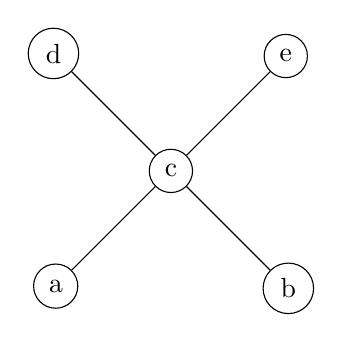
\begin{tikzpicture}[every node/.style={circle, draw}, node distance=1.5cm]
  \node (1) {c};
  \node (2) [below left=of 1] {a};
  \node (3) [below right=of 1] {b};
  \node (4) [above left=of 1] {d};
  \node (5) [above right=of 1] {e};
  
  \draw (1) -- (2);
  \draw (1) -- (3);
  \draw (1) -- (4);
  \draw (1) -- (5);
\end{tikzpicture}

\subsection{T13}
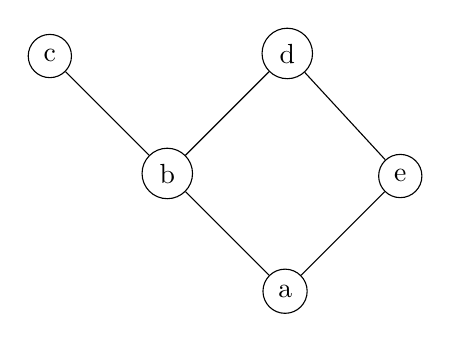
\begin{tikzpicture}[every node/.style={circle, draw}, node distance=1.5cm]
    \node (1) {a};
    \node (2) [above left=of 1]{b};
    \node (3) [above left=of 2]{c};
    \node (4) [above right=of 2]{d};
    \node (5) [above right=of 1]{e};
    \draw (1) -- (2);
    \draw (1) -- (5);
    \draw (2) -- (3);
    \draw (2) -- (4);
    \draw (5) -- (4);
\end{tikzpicture}
\subsection{T14}
\begin{tikzpicture}[every node/.style={circle, draw}, node distance=1.5cm]
    \node (1) {4};
    \node (2) [above=of 1]{3};
    \node (3) [above left=of 2] {2};
    \node (4) [above right=of 2]{5};
    \node (5) [above left=of 3]{1};
    
    \draw (1) -- (2);
    \draw (2) -- (3);
    \draw (2) -- (4);
    \draw (3) -- (5);
\end{tikzpicture}
\subsection{T16}
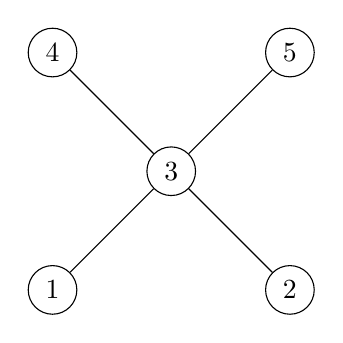
\begin{tikzpicture}[every node/.style={circle, draw}, node distance=1.5cm]
    \node (1) {3};
    \node (2) [below left=of 1] {1};
    \node (3) [below right=of 1] {2};
    \node (4) [above left=of 1] {4};
    \node (5) [above right=of 1] {5};
    
    \draw (1) -- (2);
    \draw (1) -- (3);
    \draw (1) -- (4);
    \draw (1) -- (5);
\end{tikzpicture}
  
\subsection{T18}
$
\begin{bmatrix}
    1 & 1 & 1 & 1 & 1\\
    0 & 1 & 0 & 1 & 0\\
    0 & 0 & 1 & 0 & 1\\
    0 & 0 & 0 & 1 & 0\\
    0 & 0 & 0 & 0 & 1
\end{bmatrix}
$
\subsection{T26}
(a) $\{\{1, 3, 12\}, \{2, 4\}\}$ \quad (b) $\{\{a, d, f\}, \{b, e\}, \{c\}\}$ \quad (c) $\{1, 2, 3, 4\}$\\
(d) $\{\{1, 3, 4, 6, 7, 8\}, \{2, 5\}\}$ \quad (e) $\{\{1, 2\}, \{3\}, \{4, 5, 6, 8, 9\}, \{7\}\}$
\subsection{T27}
(a) $\{2, 3\}$或$\{3, 4\}$ \quad (b) $\{a, b, c\}$ \quad (c) $\{1\}$
\quad (d) $\{2, 3\}$ \quad (e) $\{2, 3, 7, 8\}$
\subsection{T28}
相等。对于不可比的最大集合,因为该集合已经是最大的,因此其余所有图中的元素都至少与该集合中的任一元素有关系。
且因为剩余元素中不可比的最大数目小于等于最大集合内中的不可比元素数目。因此从该集合中的每个元素发散出一条链,必定可以
将其余所有元素连接起来。而每条链上的点都能组成具有全序的一个子集,且每条链之间必有一个点不相交。因此全序的子集个数与链的条数
以及最大不可比集合的基数相等。
\subsection{T29}
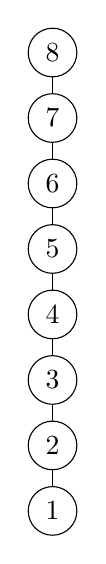
\begin{tikzpicture}[every node/.style={circle, draw}, node distance=0.2cm]
    \node (1) {1};
    \node (2) [above=of 1] {2};
    \node (3) [above=of 2] {3};
    \node (4) [above=of 3] {4};
    \node (5) [above=of 4] {5};
    \node (6) [above=of 5] {6};
    \node (7) [above=of 6] {7};
    \node (8) [above=of 7] {8};
    
    \draw (1) -- (2);
    \draw (2) -- (3);
    \draw (3) -- (4);
    \draw (4) -- (5);
    \draw (5) -- (6);
    \draw (6) -- (7);
    \draw (7) -- (8);
\end{tikzpicture}
  
\subsection{T30}
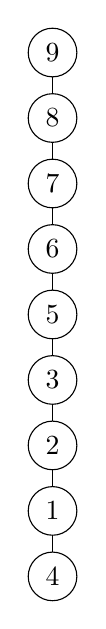
\begin{tikzpicture}[every node/.style={circle, draw}, node distance=0.2cm]
    \node (1) {4};
    \node (2) [above=of 1] {1};
    \node (3) [above=of 2] {2};
    \node (4) [above=of 3] {3};
    \node (5) [above=of 4] {5};
    \node (6) [above=of 5] {6};
    \node (7) [above=of 6] {7};
    \node (8) [above=of 7] {8};
    \node (9) [above=of 8] {9};
    \draw (1) -- (2);
    \draw (2) -- (3);
    \draw (3) -- (4);
    \draw (4) -- (5);
    \draw (5) -- (6);
    \draw (6) -- (7);
    \draw (7) -- (8);
    \draw (8) -- (9);
\end{tikzpicture}
\subsection{T34}
非自反性:$\forall a \in A$, $a < a$不成立,因此是非自反的。\\
传递性:$\forall a, b, c \in A$,当$a < b$且$b < c$时,显然有$a < c$。因此具有传递性。\\
综上所述,通常的关系$<$是$A$上的一个拟序。
\subsection{T35}
非自反性:因为$R$是$A$上的一个拟序,因此$\forall a \in A$,$(a, a) \notin R$。所以$(a, a) \notin R^{-1}$,因此是非自反的。\\
传递性:$\forall a, b, c(a, b, c \in A \land (a, b) \in R \land (b, c) \in R)$,有$(a, c) \in R$。
因此$\forall a, b, c(a, b, c \in A \land (b, a) \in R^{-1} \land (c, b) \in R^{-1})$,有$(c, a) \in R^{-1}$。因此$R^{-1}$具有传递性。\\
综上所述,$R^{-1}$也是$A$上的一个拟序。
\subsection{T36}
$R'$表示$\{(a, b) |\ a | b \land a \neq b\}$。\\
非自反性:由$R'$的定义可知,$\forall a, b$,如果$a = b$,显然$(a, b) \notin R'$,因此是非自反的。\\
传递性:因为整除本身具有传递性,故$R'$也具有传递性。\\
因此$R'$为$Z^+$上的一个拟序。
\subsection{T38}
自反性:对于任意二阶布尔矩阵$M$,一定有$m_{ij} = n_{ij}, 1\leq i \leq 2, 1 \leq j \leq 2$。因此$R$满足自反性。\\
反对称性:$\forall M, N \in A, M \neq N \land M R N$。则必定存在$m_{ij} < n_{ij}$。因此$n_{ij} > m_{ij}$,所以$(N, M) \notin R$,因此$R$满足反对称性。\\
传递性:因为运算$\leq$具有传递性,因此$\forall M, N, O \in A, (M, N) \in R \land (N, O) \in R$,即$\forall i, j (m_{ij} \leq n_{ij}) \land (n_{ij} \leq o_{ij}) \rightarrow (m_{ij} < o_{ij})$。
故$(M, O) \in R$,因此满足传递性。\\
综上所述,因为$R$满足自反性、反对称性、传递性,因此$R$是$A$上的一个偏序。
\subsection{T40}
对于$(A, \leq)$,因为$1 | 2 \land 2 | 4 \land 4 | 8$,因此$(A, \leq)$是一个全序关系。
对于$(A', \leq')$,因为$0 \leq 1 \leq 2 \leq 3$,所以$(A', \leq')$也是一个全序关系。
因为$(A, \leq),(A', \leq')$都是全序关系并且元素都为4个,因此必定同构。
\section{6.2}
\subsection{T6}
\subsection{T8}
\subsection{T12}
\subsection{T14}
\subsection{T17}
\subsection{T18}
\subsection{T19}
\subsection{T20}
\subsection{T22}
\subsection{T23}
\subsection{T24}
\subsection{T25}
\subsection{T26}
\subsection{T32}
\subsection{T33}
\subsection{T35}
\subsection{T36}
\subsection{T37}
\subsection{T38}
\section{6.3}
\subsection{T1}
\subsection{T2}
\subsection{T3}
\subsection{T4}
\subsection{T5}
\subsection{T6}
\subsection{T13}
\subsection{T14}
\subsection{T15}
\subsection{T18}
\subsection{T19}
\subsection{T20}
\subsection{T22}
\subsection{T24}
\subsection{T25}
\subsection{T26}
\subsection{T27}
\subsection{T29}
\subsection{T34}
\subsection{T37}
\subsection{T38}
\subsection{T39}
\subsection{T40}
\end{document}
